\documentclass[11pt,leqno]{book}
\textwidth 13.5cm
\textheight 18.5cm
\topmargin 0in
\parindent 0.5cm
\oddsidemargin 0.5in
\evensidemargin 0.5in
\usepackage{amssymb}
\usepackage{amsmath}
\usepackage{graphicx,wrapfig,url,rotating,array}
\usepackage{fan}
%
\def\bibname{{\Large\bf References}}
\def\thebibliography#1{\addvspace{3em}\noindent
\noindent \bibname  \list
 {[\arabic{enumi}]}{\settowidth\labelwidth{[#1]}\leftmargin\labelwidth
 \advance\leftmargin\labelsep
 \usecounter{enumi}}
 \def\newblock{\hskip .11em plus .33em minus .07em}
 \sloppy\clubpenalty4000\widowpenalty4000
 \sfcode`\.=1000\relax}
\let\endthebibliography=\endlist
%
\usepackage[english]{babel}
%
\pagestyle{fancy}
\footrulewidth 0pt
\headrulewidth 0.5pt
\lfoot[\thepage]{} \cfoot[]{} \rfoot[]{\thepage}
\lhead[Geometric Visualization of a Polygon Area Partitioning]{ESGI'132} \chead[]{} \rhead[ESGI'132]{Geometric Visualization of a Polygon Area Partitioning}
%
\def\efig#1#2{\includegraphics[width=#2mm]{#1}}
\def\efigsc#1#2{\includegraphics[scale=#2]{#1}}
\def\TTT{\end{document}}
\def\bt{\begin{tabular}}
\def\et{\end{tabular}}
\def\cl{\centerline}
\def\mc{\multicolumn}
%
\def\diag{\mathop{\rm diag}}
\thispagestyle{empty}
\newcommand{\sect}[1]{\vskip7mm\par{\large \bf #1}}
\newcommand{\subsect}[1]{\vskip 3mm\par{\bf#1}}
%
 \def\hlst{\setlength{\topsep}{1pt}\setlength{\partopsep}{1pt}%
 \setlength{\parsep}{1pt}\setlength{\itemsep}{\parskip}}
%
\begin{document}
%
\begin{center}
\textbf{\LARGE Geometric Visualization of a Polygon Area Partitioning}

\vspace*{5mm}
%
Todor Balabanov,
Stanislav Darachev,
Ivan Jordanov,
Aleksandar Karakushev,
Nikolai Kitanov,
Alexander Manov,
Georgi Nikolov,
Spasimir Nonev,
Zdravka Nedyalkova,
Emiliyan Rogachev,
Natasha Stojkovikj,
Petar Tomov,
Iliyan Zankinski
%
\end{center}
%
\date{18-22 Sep 2017}
%
\sect{Abstract}
%
In the process of modeling sewerage networks, the main component is the drained area (catchment) from which water is collected to each conduit (pipe). If the area for a single subcatchment is derived from a mathematical model, we have to create the geometry of that territory. For visualization purpose, we need to find geometric partitioning of the polygon.

In this paper we propose 6 solutions for geometric visualization of a polygon area partitioning.

\textit{Key words}: visualization, polygon area partitioning, optimal cutting problem

\sect{1.~Introduction}

The problem  mathematically is formulated in the following way:

A polygon $P$ (corresponding to the catchment) is given with the Cartesian coordinates of its vertices (corresponding to Manholes) and its edges $i= 1, \ldots, N$, (corresponding to pipes). Thus, the area of the polygon $F$ is also known. With each edge, we associate a relative area $f_i$ (corresponding to the relative water debit in percentages), where  $100\% = \sum f_i$.

\begin{center}
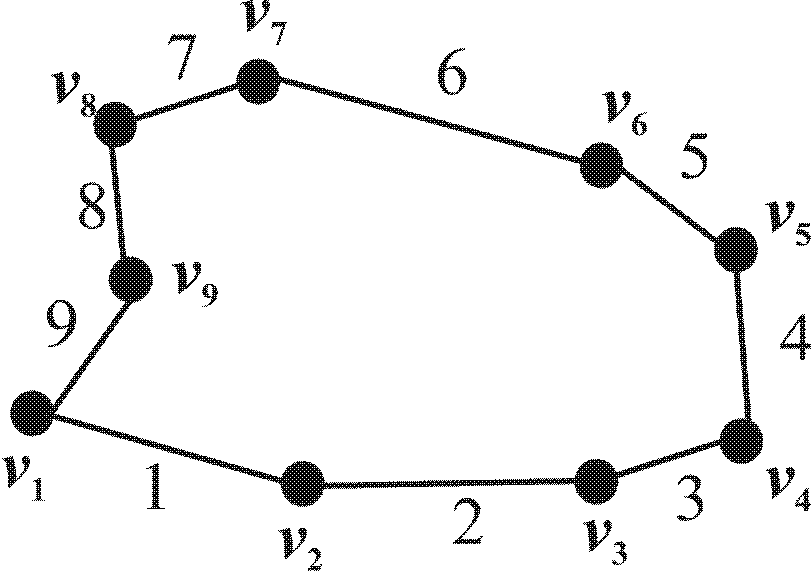
\includegraphics  {pic01.png}

Fig. 1.Polygon
\label{fig1}
\end{center}

The vertices of the polygon are denoted with $v_i$, $ i = 1, \ldots, N$.
For visualization purposes, we look for a geometric partitioning of the polygon, such that the area of the$i$-th part is equal to $f_i$.

For the given  data  in Table 1.

\begin{table}[h!]
\begin{center} \scriptsize{
\begin{tabular}{|c|c|}
\hline
 i & $f_i(\%)$ \\
\hline
 1 & 23,93 \\
\hline
 2 & 24,21 \\
\hline
 3 & 3,23  \\
\hline
 4 & 6,88 \\
\hline
 5 & 7,00 \\
\hline
 6 & 15,63  \\
\hline
 7 & 6,40 \\
\hline
 8 & 5,15 \\
\hline
 9 & 7,68  \\
\hline
 F & 1 \\
  \hline
\end{tabular}
}
\resizebox{1\textwidth}{!}{\begin{minipage}{\textwidth}
\caption{Given data}
\end{minipage}}
\end{center}
\end{table}

Standard visual interpretation is given in Fig.2.

\begin{center}
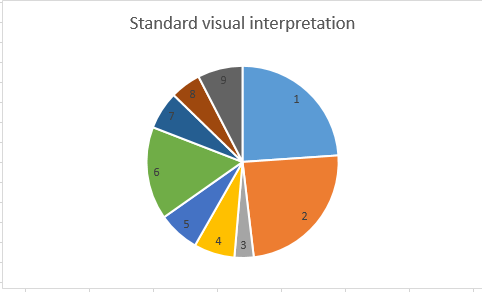
\includegraphics  [scale=0.58] {pic02.png}

Fig. 2.{Standard visual interpretation}
\label{fig2}
\end{center}

We looking for the following visual (geometrical) interpretation (Fig.3)

\begin{center}
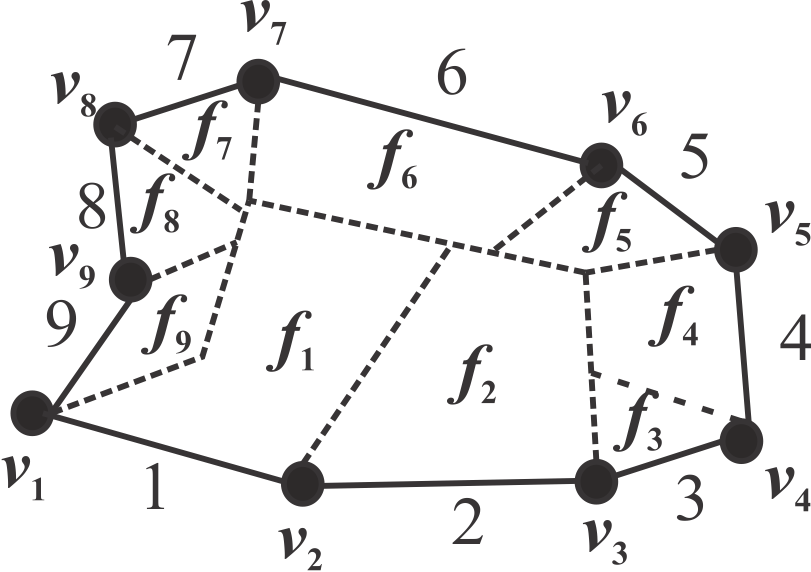
\includegraphics  {pic03.png}

Fig. 3.{Visaul geometrical interpretation}
\label{fig3}
\end{center}

\sect{2.~Solution approaches}

\subsect{2.1.~Monte Carlo Flooding Algorithm}

With this algorithm the polygon will be divided in $N$ irregular shapes. Let the area of the figures is noticed by $c_i, i = 1. \ldots, N$.  Following is the pseudocode of the proposed MCFA.

\noindent\rule{\textwidth}{1pt}
\begin{itemize}
\item[Step 1.]  For all edges, find middle point of the edge, $t_i(x,y)$.
\item[Step 2.]  For all points $t_i(x,y), i=1,\ldots, N$, form figures $IF_i$ from the nearest points on the point $t_i(x,y)$. 
\item[Step 3.] Find areas of the formed figures, $c_i, i = 1, \ldots, N$.
\item[Step 4.] For $i = 1$ to $N$
\begin{itemize}
  \item[Step 4.1]  While ($c_i \leq f_i$)
  \item[Step 4.2]  Add nearest points to boundary on figure $IF_i$ in the figure $IF_i$. 
\end{itemize}
\end{itemize}
\noindent\rule{\textwidth}{1pt}

The final result of the algorithm is similar to liquid foolding from different sides.

\subsect{2.2.~Genetic Algorithm}

First, we choose $N$ point, $b_i$  on random way, where $N$ is a number of edges.

\begin{center}

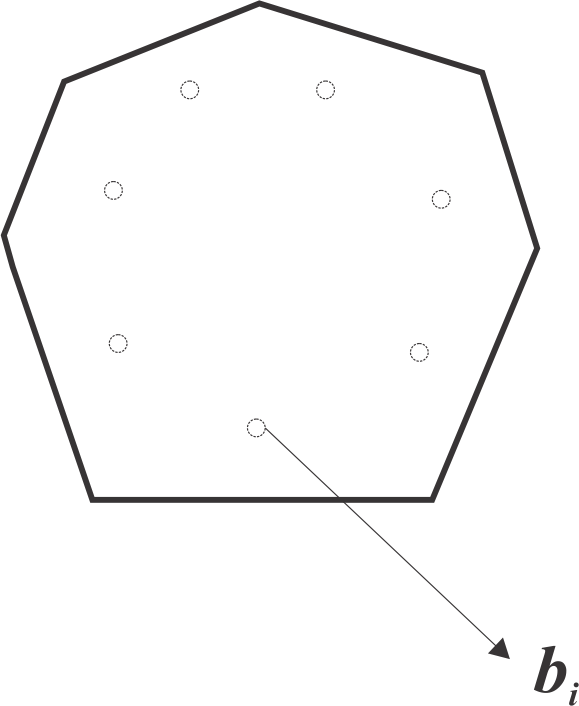
\includegraphics {pic04.png}

Fig. 4.
\label{fig4}
\end{center}.

Each of these points, with the end points from the edges of the polygon will be connected, and on this ways we form $N$ triangles  $T_i$. The area of the triagles $T_i, i=1, \ldots, N $ will be denoted with $a_i$. The area of the polygon, outside of the triangles is denoted with $W$.  This is shown on Fig 5.

\begin{center}
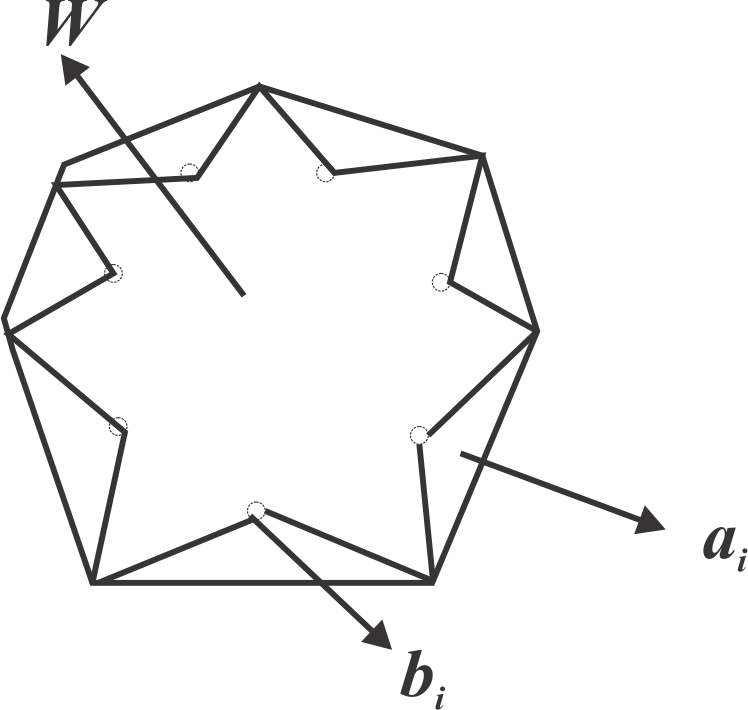
\includegraphics{pic05.png}

Fig. 5.
\label{fig5}
\end{center}.

We form following sums:
$$B= count( b_i), i =1, \ldots, N$$
$$ W= count(w_{(x,y)})$$ where $w_{ (x,y)}\notin T_i, \forall{ T_i}, i=1, \dots, N$
$$ A= \sum_{(a_i - f_i)>0}(a_i-f_i)$$
Now, we regard one triangle.  Let, for the random point $t(x_i, y_i) \in T_i$,  $d_{ij}$  is distance from the point to the $i$-edge from the polygon. 

\begin{center}
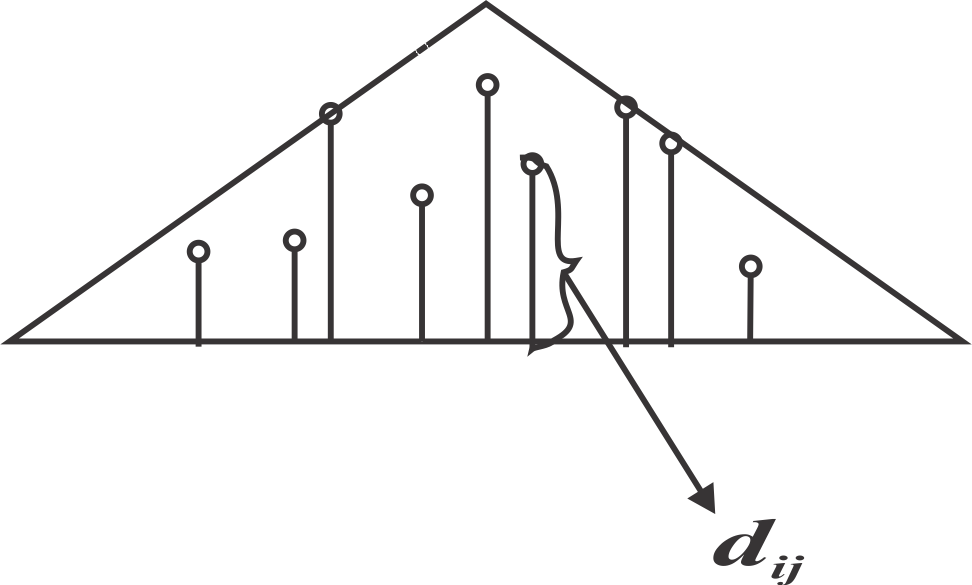
\includegraphics{pic06.png}

Fig. 6.
\label{fig5}
\end{center}

The  following sums are formed: $$d_i = \frac{\sum_{j=1}^k d_{ij}}k$$
where $k$ is a  total number of the point on the triangle  and

$$D = \sum_{i=1}^N d_i$$.

We need to estimated cost function
$$cost f = D+W + A + B$$.

Our goal is to minimized the cost function. Since, we need to minimize $D, W, A, B$. The set of values for $W$ is $[0, count( p(x_i, y_i))], \forall p(x_i, y_i) \in P$. From , this we can conclude, that optimal value for W is 0.
The set of values for $A$ is $[0, count (p(x_i, y_i))], \forall p(x_i, y_i) \in P$, we conclude that minimal value of $A$ is 0. And, the $B$ have set of values $[N,count( p(x_i, y_i))], \forall p(x_i, y_i) \in P$, and minimal value from $B$ is $N$, where $N$ is a number of edges of the polygon.
if we succeed to minimize $A, B, W$, we will give the minimum value of the cost function.

\subsect{2.3.~Percent Distributed Clustering}

The given area is divided into a fine grid of pixels. The sides of the polygon are also divided into sixty line segments each. For each pixel of the area the algorithm finds the line segment that gives the lowest value for the distance between the pixel and the line segment multiplied by 100 minus the required percentage of the area: distance * (100 - f(x)). The side that the line segment belongs to is the side that the area taken by the pixel will drain into.

\subsect{2.4.~Offsetting Polygon}

\noindent\rule{\textwidth}{1pt}
\begin{itemize}
\item[Step 1.] Draw a parallel segment to each side of the polygon, creating a smaller polygon inside. 
\item[Step 2.] Connect each of the corresponding vertices of each polygon and calculate the area of the trapezoids created.
\item[Step 3.] Calculate the area of the created trapezoids and check if it fits the data.
\item[Step 4.] If the area doesn’t fit we continue with creating parallel polygons.
\begin{itemize}
  \item[Step 4.1] If the desired area is accomplished, fix the side of the corresponding trapezoid and stop drawing parallel sides for it.
  \item[Step 4.2] 
\end{itemize}
\end{itemize}
\noindent\rule{\textwidth}{1pt}

After we are done with 4.2 we simplify the polygon on which we run the algorithm. Following these iterations we get a triangle(s) in the end which area to side distributions we can find easily.

\subsect{2.5.~Fifth approach}

\subsect{2.6.~Sixth approach}

\sect{3.~Experimens and Results}

\subsect{3.1.~Monte Carlo Flooding Algorithm}

\subsect{3.2.~Genetic Algorithm}

\subsect{3.3.~Percent Distributed Clustering}

\subsect{3.4.~Offsetting Polygon}

\subsect{3.5.~Fifth approach}

\subsect{3.6.~Sixth approach}

\sect{Conclusions}

\sect{Acknowledgements}

\def\bibname{{\Large\bf References}}
\begin{thebibliography}{99}
%
\bibitem{1} ....
%
\bibitem{2} ....
%
\end{thebibliography}
%
\end{document}
